% Number squares paper for 18.821 Fall 2012 project 2.
% Authors: Daniel Grazian, Michael Mekonnen, Agustin O Venezuela III

\documentclass[12pt]{amsart}

% Keep everything here in alphabetical order, please! :) -jven

% Packages

\usepackage{amssymb}
\usepackage{graphicx}

% Enumeration

\newtheorem{theorem}{Theorem}[section]

\newtheorem{conjecture}[theorem]{Conjecture}
\newtheorem{corollary}[theorem]{Corollary}
\newtheorem{definition}[theorem]{Definition}
\newtheorem{example}[theorem]{Example}
\newtheorem{examples}[theorem]{Examples}
\newtheorem{lemma}[theorem]{Lemma}
\newtheorem{proposition}[theorem]{Proposition}
\newtheorem{remarks}[theorem]{Remarks}
\newtheorem{remark}[theorem]{Remark}

% Utility commands

% vspace
\newcommand{\breathe}{\vspace{0.2cm}}
% xor
\newcommand{\xor}{\oplus}
% Integers
\newcommand{\z}{\mathbb{Z}}
% Our 'difference' operation
\newcommand{\diff}{D}
% Non-negative integers
\newcommand{\znn}{\mathbb{N}}
% Positive integers
\newcommand{\zp}{\mathbb{Z}^+}

\title{Number Squares}
\author{Daniel Grazian, Michael Mekonnen, Agustin O Venezuela III}
\date{October 23, 2012}

\begin{document}

\begin{abstract}
We investigate the behavior of an operator that maps tuples to same-size tuples, seeking to characterize those starting tuples which, upon successive applications of the operation, yield the zero tuple in finite time.
\end{abstract}

\maketitle

\section{Introduction\label{sec:intro}}

In this paper, we present an operation $\diff$ that acts on tuples of integers in a very simple way. Given a 4-tuple (a, b, c, d):

$$\diff((a, b, c, d)) = (|a - b|, |b - c|, |c - d|, |d - a|).$$ 

For example:

$$\diff((2, 6, 1, 9)) = (4, 5, 8, 7).$$

In particular, we are interested in repeatedly applying $\diff$ to an initial tuple, until the tuple (0, 0, 0, 0) is reached (if it is ever reached at all.) We call the (possibly infinite) sequence of tuples obtained by repeatedly applying $\diff$ to $(a, b, c, d)$ until (0, 0, 0, 0) is reached  the $(a, b, c, d)$ \textit{game} or, where the context is clear, simply $(a, b, c, d)$.

For example, the  $(3, 7, 2, 5)$ game is:
\begin{align*}
& (3, 7, 2, 5) \\
& (4, 5, 3, 2) \\
& (1, 2, 1, 2) \\
& (1, 1, 1, 1) \\
& (0, 0, 0, 0)
\end{align*}

This particular game takes 4 steps (applications of $\diff$) to terminate and includes 5 tuples, so we say it has length 5. The table in Figure \ref{fig: lengthVersusStartingTuple} gives the lengths of several other games. The entries of the starting tuples were selected uniformly at random from $0$ to $1000$.

\begin{figure}
\caption{Length of game versus starting tuple}
\label{fig: lengthVersusStartingTuple}
\begin{center}
    \begin{tabular}{| c | c |}
    \hline
    Starting tuple &  Length of game\\ \hline
    (540, 752, 144, 4) & 5\\ \hline
    (345, 906, 136, 149) & 7\\ \hline
    (912, 135, 490, 150) & 5\\ \hline
    (129, 660, 348, 211) & 8 \\ \hline
    (215, 57, 594, 502) & 6 \\ \hline
    \end{tabular}
\end{center}
\end{figure}

This table may seem rather surprising. Apparently, typical games terminate, and furthermore, they terminate in very few steps. This observation is definitely not immediately obvious from the definition of $\diff$, and it provides motivation for this paper, which is devoted to investigating the lengths of games and the conditions under which games terminate. 

%First, we generalize the operation $\diff$ in the natural way to tuples of sizes other than $4$. In particular, given a k-tuple $(a_0, \ldots, a_{k-1})$:
%
%$$\diff(a_0, \ldots, a_{k-1}) = (|a_0 - a_1|, |a_1 - a_2|, \ldots, |a_{k-2} - a_{k-1}|, |a_{k-1} - a_0|).$$
%
%For example:
%
%$$\diff((4, 12, 1, 0, 5, 7)) = (8, 11, 1, 5, 2, 3).$$
%
%$\diff$ can also be applied analogously to tuples of real numbers. For example:
%
%$$\diff(\pi, 1, 3, \sqrt{2}) = (\pi - 1, 2, 3 - \sqrt{2}, \pi - \sqrt{2}).$$

In Section \ref{sec:invariants} we show that the length of a game is invariant under certain operations on the starting tuple. This simplifies our analysis in the remaining sections.

In Section \ref{sec:convergence} we show that every 4-tuple game over the integers does indeed terminate in a finite number of steps, as suggested by the table in Figure \ref{fig: lengthVersusStartingTuple}. We also provide an upper bound on the number of steps required for such a game to terminate, in terms of the entries of the starting tuple.

In Section \ref{sec:longgames}, however, we show that it is possible to construct a 4-tuple game over the integers of arbitrarily long finite length. 

In Section \ref{sec:othertuples} we analyze games with tuples of sizes other than $4$. We show that for every $k > 2$, if $k$ is an integer power of 2 (such as 2, 4, 8, etc.), then every $k$-tuple game over the integers terminates in a finite number of steps. We also show that if $k$ is not an integer power of 2, then there exist $k$-tuple games over the integers that do \textit{not} terminate in a finite number of steps (that is, that never reach (0, \ldots, 0)).

Finally, in Section \ref{sec:nonIntegers} we extend our analysis beyond the integers. We show that all 4-tuple games on the rational numbers terminate in a finite number of steps (just as was the case for the integers.) Additionally, we exhibit a large class of 4-tuple games on the real numbers that terminate quickly. However, we also construct a 4-tuple game on the real numbers that never terminates.

%Our aim is to completely understand the behavior of this operation under various starting tuples. Specifically, we are interested in applying the difference to a given tuple successively until a tuple of all zeroes is reached, or else concluding that the zero tuple will never be reached.
%
%Our analysis has resulted in a number of observations. First, for any starting tuple whose size is of the form $2^k$, the difference eventually yields the same-size tuple of all zeroes after finitely many steps. We also provide an upper bound on the number of applications of the difference that are necessary for a given starting tuple. On the other hand, we also show that there exist games of arbitrarily long finite length. Second, we show that this does not hold for tuple sizes not of the form $2^k$: that is, we can construct such tuples so that upon successive applications of the difference, the zero tuple is never reached. We finally extend the notion of the difference to operate on tuples of non-integers, also with the aim of understanding which starting tuples eventually yield the zero tuple.
%
%We will begin by presenting the definition of the difference in the context of $4$-tuples of integers. The $4$-tuple case completely captures the problem for all $2^k$-tuples so it is useful to begin here. Next, we give a construction for infinitely long games for all tuple sizes not of the form $2^k$. We then present the details for generalizing our arguments for $4$-tuples to $2^k$-tuples. Finally, we address the extension of the difference operator to tuples over $\mathbb{Q}$ and $\mathbb{R}$.
%
%\section{Definitions and Notation\label{sec:defs}}
%
%We will now define the operation that was introduced in the previous section. Herein, we will use $\znn$ to denote the non-negative integers and $\zp$ to denote the positive integers. Also, at times when we feel it will promote clarity and ease of understanding, we will abuse the notation $n\pmod{m}$ and mean the remainder of $n$ upon division by $m$.
%
%\begin{definition}
%Given a $4$-tuple $(a, b, c, d)\in \mathbb{Z}^4$, the \underline{difference} $D((a, b, c, d))$ of $(a,b,c,d)$ is the $4$-tuple $(|a - b|, |b - c|, |c - d|, |d - a|)$.
%\end{definition}
%
%As motivated in the introduction, we are interested in repeatedly applying the difference to a $4$-tuple until we reach the tuple consisting of all zeroes. In particular, we have the following definition:
%
%\begin{definition}
%Given a $4$-tuple $(a, b, c, d)\in \mathbb{Z}^4$, the \underline{(a, b, c, d) game} is the (possibly infinite) sequence of $4$-tuples $\big((a_i, b_i, c_i, d_i)\big)$, generated as follows:
%
%\begin{enumerate}
%\item $(a_0, b_0, c_0, d_0) = (a, b, c, d)$
%\item $\forall i\in \znn$, if $(a_i, b_i, c_i, d_i) = (0, 0, 0, 0)$, then the $(a, b, c, d)$ game is a finite sequence ending at $(a_i, b_i, c_i, d_i)$. Otherwise:
%
%$$(a_{i+1}, b_{i+1}, c_{i+1}, d_{i+1})=D((a_i, b_i, c_i, d_i)).$$
%\end{enumerate}
%\breathe
%We will often refer to a $4$-tuple as a game itself, where it is understood that we mean the game whose first element is this $4$-tuple.
%
%\end{definition}
%
%Note that by this definition, the game of a $4$-tuple is either finite ending in $(0, 0, 0, 0)$ or infinite and never containing $(0, 0, 0, 0)$. Naturally, we will refer to the length of a game, meaning the (possibly infinite) length of the sequence.

\section{Simplifying Observations\label{sec:invariants}}

In this section, we aim to make observations that will simplify our analysis in the rest of the paper.

First, we list three operations on the starting tuple of a game under which the length of the game is invariant. We will use these operations throughout the paper to make simplifying modifications to games without affecting their lengths. Suppose $(a_0, a_1, \dots, a_{k-1})$ is a game of length greater than $2$. Now we can make the following assertions:

\begin{enumerate}
\item The $(a_1,a_2, \dots, a_{k-1}, a_0)$ game has the same length. That is, cyclically permuting a tuple does not change the length of the game. Each tuple in the $(a_1,a_2, \dots, a_{k-1}, a_0)$ game contains the same elements as the corresponding tuple in the $(a_0, a_1, \dots, a_{k-1})$ game, except cyclically shifted left by $1$. \\
\item The $(ua_0, ua_1, \dots, ua_{k-1})$ game, for any $u \in \mathbb{R} - \{0\}$, has the same length. That is, scaling a tuple by a non-zero number does not change the length of the game. The subsequent tuples in the $(ua_0, ua_1, \dots, ua_{k-1})$ game are the same as the corresponding tuples in the $(a_0, a_1, \dots, a_{k-1})$ game, except scaled by $|u|$. \\
\item The game $(a_0 + v, a_1 + v, \dots, a_{k-1} + v)$, for any $v \in \mathbb{R}$, has the same length. That is, translating a tuple does not change the length of the game. After one step, the games $(a_0, a_1, \dots, a_{k-1})$ and $(a_0 + v, a_1 + v, \dots, a_{k-1} + v)$ will be identical.
\end{enumerate}

Second, we will assume that all starting tuples for the games we consider contain only non-negative elements. The reason for this is that, regardless of the elements in the first tuple, the second tuple of the game will contain only non-negative elements. So if we are interested in studying a game that starts with a tuple $(a_0, a_1, \dots, a_k)$ containing negative elements, we can just consider the game starting from $\diff((a_0, a_1, \dots, a_k))$.

\section{Finiteness of All Games\label{sec:convergence}}

We will now show that every integer $4$-tuple game terminates at the $4$-tuple $(0,0,0,0)$ in finite time (actually, as we will see, very quickly).

The main result we shall use to prove this claim is the following.
\begin{theorem}
For any $a,b,c,d \in \z$ and $n \in \znn$, the $4$-tuple $\diff^{4n}((a, b, c, d))$ has elements that are all congruent to $0\pmod{2^n}$.
\label{thm:pow2}
\end{theorem}

\begin{proof}
We prove this by induction on $n$.

The base case for which $n=0$ follows trivially because it simply asserts that $a$, $b$, $c$, and $d$ are congruent to $0\pmod{1}$.

In the inductive step, we need to show that for any $n \in \znn$, if $a$, $b$, $c$, and $d$ are congruent to $0\pmod{2^n}$, then $\diff^4((a, b, c, d))$ will have elements that are congruent to $0\pmod{2^{n+1}}$. Before proving this, let us make an important observation.

For any $a$, $b$, $c$, $d$, we have that $\diff^4((a,b,c,d))$ contains only even elements. To prove this, it suffices to show that any game that starts with a $4$-tuple only containing $0$s and $1$s terminates after $4$ steps. Indeed, there are $16$ $4$-tuples that contain only $0$s and $1$s, but we only need to consider $6$ of them, namely $(0,0,0,0)$, $(0,1,1,1)$, $(1,0,0,0)$, $(1,0,0,1)$, $(1,0,1,0)$, and $(1,1,1,1)$, since the other $10$ $4$-tuples can be obtained by appropriate cyclic permutation of one of these $6$. Since the length of a game is invariant under cyclic permutations, studying these $6$ $4$-tuples is sufficient. Figure \ref{fig:zerosones} shows a graph in which the nodes represent the $6$ $4$-tuples we are studying, and an edge from node $A$ to node $B$ indicates that $B = \diff(A)$. From this graph, it is clear that all of the games have finite length. Furthermore, the maximum number of steps necessary for termination is $4$, achieved, for example, by $(1,0,0,0)$).

\begin{figure}
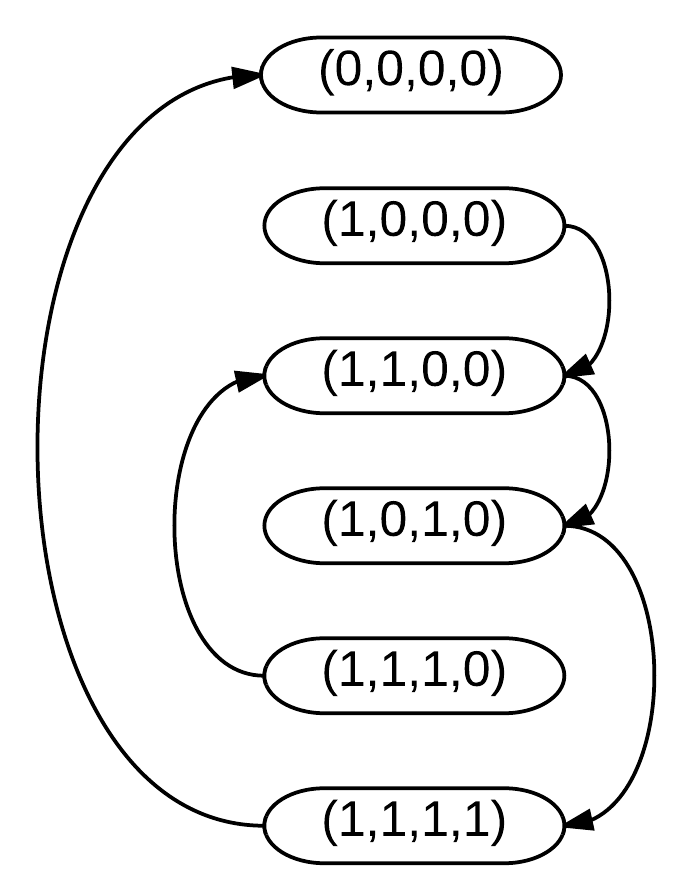
\includegraphics{number_squares_0s_and_1s.png}
\caption{All games starting with just $0$s and $1$s have length at most $5$.}
\label{fig:zerosones}
\end{figure}

Returning to the proof of the inductive hypothesis, we note that we can take out a factor of $2^n$ from the $(a,b,c,d)$ game since $a$, $b$, $c$, and $d$ are congruent to $0\pmod{2^n}$. If we take $4$ steps while keeping the $2^n$ factored out, we have that the remaining values must be even, which shows that the elements of $\diff^4(a,b,c,d)$ are congruent to $0\pmod{2^{n+1}}$. This concludes the inductive proof.

\end{proof}

\begin{corollary}
Let $M=\max(a,b,c,d)$. Then the game $(a,b,c,d)$ is finite and has length at most $4(\lfloor\log_2{M}\rfloor + 1) + 1$.
\end{corollary}

\begin{proof}
Let $n = \lfloor\log_2{M}\rfloor + 1$. By Theorem \ref {thm:pow2}, $\diff^{4n}((a, b, c, d))$ has elements that are congruent to $0\pmod{2^n}$. However, since $M < 2^n$, all of the elements in $\diff^{4n}((a, b, c, d))$ are also less than $2^n$, and thus are all zero.
\end{proof}

\section{Existence of Arbitrarily Long Finite Games\label{sec:longgames}}

The previous section argued that all games are of finite length. However, we will show in this section that games may be of any arbitrarily long finite length. We state this more precisely in the following theorem:

\begin{theorem}
For all $n\in \zp$, there exists a game of length $n$.
\end{theorem}

For $n < 5$, it is very easy to construct such a game. Indeed, for $n=1,2,3,4$ we have the games $(0, 0, 0, 0)$, $(1, 1, 1, 1)$, $(1, 0, 1, 0)$, and $(1, 1, 0, 0)$, respectively.

Our plan for $n \geq 5$ is as follows: given games of a particularly nice form, we will show how to construct a game of one greater length while still preserving this form. The result is that this construction can be repeated indefinitely until a game of the desired length is reached.

Suppose there exists a game $(0, a, b, c)$ of length $n$, where $0\leq a\leq b\leq c$ and $a + b < c$. Alter this game by doubling each element, then adding $c - b - a$ to each element. This yields the game:

$$\begin{array}{cl}
& (c - b - a, 2a + (c - b - a), 2b + (c - b - a), 2c + (c - b - a)) \\
= & (-a - b + c, a - b + c, -a + b + c, -a - b + 3c)
\end{array}$$

We showed in Section \ref{sec:invariants} that game length is invariant under scaling as well as addition of each element in the tuple by a constant. Thus this game also has length $n$. Furthermore, since each element of this tuple is non-negative (and in fact positive), it is the sequence obtained by applying $\diff$ to the following sequence:

$$(0, -a - b + c, -2b + 2c, -a - b + 3c)$$

This game thus has length $n + 1$. Note also that this tuple is again of the form $(0, a', b', c')$, where $0\leq a'\leq b'\leq c'$ and $a' + b' = -a - 3b + 3c < -a - b + 3c = c'$. Thus we may iterate this process to yield a game of length $n + 2$, and so on.

It thus remains to provide a game of length $5$ and of the form $(0, a, b, c)$, $0\leq a\leq b\leq c$, $a + b < c$, since all subsequent game lengths can be obtained by iterating the above process repeatedly from such a game. The game $(0, 1, 1, 3)$ is of the desired form and has length $5$, so we're done. $\qed$

Note that our proof is constructive: given any $n\in \zp$, the proof gives an algorithm to find a length $n$ game. As an example, starting with the length $5$ game $(0, 1, 1, 3)$, we find that a length $50$ game is:

$$(0, 103502633381134336, 293873656088494080, 644020556730990592)$$

\section{Games For Other $k$-tuples\label{sec:othertuples}}

We now extend our discussion to games with tuples of sizes other than 4. We generalize the operation $\diff$ to act in the natural way on tuples of other sizes. In particular, given a k-tuple $(a_0, \ldots, a_{k-1})$:

$$\diff(a_0, \ldots, a_{k-1}) = (|a_0 - a_1|, |a_1 - a_2|, \ldots, |a_{k-2} - a_{k-1}|, |a_{k-1} - a_0|)$$.

For example:

$$\diff((4, 12, 1, 0, 5, 7)) = (8, 11, 1, 5, 2, 3)$$.

We show that given $k > 2$, if $k$ is an integer power of $2$ (1, 2, 4, etc.), then every $k$-tuple over the integers terminates in a finite number of steps. Otherwise, there exist $k$-tuple games over the integers of infinite length.

\subsection{Finiteness of All $2^k$-tuple Games}

We now show that all games of $2^k$-tuples are of finite length.

\begin{theorem}
For $k\in \znn$, all games of $2^k$-tuples are finite.
\end{theorem}

Our proof strategy is the same as that of the original $4$-tuple case. We will show that given any initial tuple, after $2^k$ steps, each element of the tuple will be congruent to $0\pmod{2}$, and thus congruent to either $0$ or $2\pmod{4}$. But then after another $2^k$ steps, each element of the tuple will be congruent to $0\pmod{4}$, and so on. Now let $B$ be the maximal element of the starting tuple. (Just as in the $4$-tuple case, we assume with no loss of generality that the starting tuple consists only of non-negative integers.) Choosing $e$ so that $2^e>B$, it is clear that after $2^ke$ steps, all elements of the tuple will be congruent to $0\pmod{2^e}$, and thus equal to $0$, as desired.

The only statement in our proposed strategy that does not obviously generalize from our proof in the $4$-tuple case is the fact that any game for a $2^k$-tuple of $0$s and $1$s is finite and of length at most $2^k+1$. It thus suffices to prove this statement. We will do so by finding a binary operation (a ``sum'') on these tuples of $0$s and $1$s that commutes with $\diff$. We will next construct a ``basis'' of such tuples whose games are known to be of finite length. Finally, we exhibit that all tuples of $0$s and $1$s can be expressed as a sum of tuples in this basis. The commutativity of the operators then allows us to conclude that all tuples of $0$s and $1$s yield games of finite length.

\begin{definition}
Let $(a_i),(b_i)$ be $n$-tuples whose elements are $0$ or $1$. The \textbf{exclusive or} $(a_i)\xor (b_i)$ (herein referred to as \textbf{xor}) is the $n$-tuple whose $i^{th}$ element is $(a_i+b_i)\pmod{2}$. For example, $(0,1,0,1)\xor(0,0,1,1)=(0,1,1,0)$. It is clear that $\xor$ is commutative and associative.
\end{definition}

We now show that xor commutes with $\diff$.

\begin{lemma}
Let $(a_i),(b_i)$ be $n$-tuples whose elements are $0$ or $1$. Then $\diff((a_i)\xor (b_i))=\diff((a_i))\xor \diff((b_i))$.
\end{lemma}

\textit{Proof}: The key observation is that when $u,v\in \{0,1\}$, $|u-v|=(u+v)\pmod{2}$. We have that the $i^{th}$ element of $\diff((a_i)\xor (b_i))$ is

$$\begin{array}{cl}
& |(a_i+b_i)\pmod{2} - (a_{i+1}+b_{i+1})\pmod{2}| \\
= & (a_i+a_{i+1}+b_i+b_{i+1})\pmod{2}
\end{array}$$

(In the case $i=n-1$, take $i+1$ to be $0$.) The $i^{th}$ element of $\diff((a_i))\xor \diff((b_i))$ is

$$\begin{array}{cl}
& (|a_i-a_{i+1}|+|b_i-b_{i+1}|)\pmod{2} \\
= & (a_i+a_{i+1}+b_i+b_{i+1})\pmod{2}
\end{array}$$

The result follows. $\qed$

We now construct a set of $2^k$-tuples over $\{0,1\}$ such that (i) all tuples in the set yield games of finite length and (ii) any $2^k$-tuple over $\{0,1\}$ can be written as the xor of tuples in the set.

\begin{lemma}
The game for any $2^k$-tuple consisting of $2^k-1$ $0$s and one $1$ is finite and of length $2^k+1$.
\end{lemma}

\begin{proof}
We need only show that this holds for the tuple $(0,0,\ldots,0,1)$. The other such tuples follow by the fact that game length is invariant under cyclic permutation of tuples, as demonstrated in Section $\ref{sec:convergence}$.

We proceed by induction on $k$. We strengthen our induction hypothesis by not only requiring that the game $(0,0,\ldots,0,1)$ is finite and of length $2^k+1$ but also that a $1$ does not appear as the first element until the penultimate tuple $(1,1,\ldots,1,1)$. For $k=0$, the game $(1)$ is $((1),(0))$, which is of length $2=2^0+1$, and trivially does not have a $1$ as the first element until the penultimate tuple $(1)$.

Now suppose the result holds for some $k\in \znn$ and consider the $2^{k+1}$-tuple game $(0,0,\ldots,0,0,0,0,\ldots,0,1)$. Note that throughout the game, the last $2^k$ elements of the tuple will proceed as the $2^k$-tuple case so long as the first element of the tuple is $0$ and that the first $2^k$ elements of the tuple will remain $0$ until the $(2^k+1)^{th}$ element (the first element of the second half) is $1$. By our induction hypothesis, we have both of these guarantees, so that after $2^k-1$ steps, the tuple is $(0,0,\ldots,0,0,1,1,\ldots,1,1)$. After one more step, we have $(0,0,\ldots,0,1,0,0,\ldots,0,1)$. Now again, the first $2^k$ elements and the last $2^k$ elements will each proceed as in the $2^k$-tuple case so long as the first and $(2^k+1)^{th}$ elements are $0$. By the induction hypothesis, we again have this, so that after a total of $2^{k+1}-1$ steps, we have $(1,1,\ldots,1,1,1,1,\ldots,1,1)$. One more step yields the zero tuple, after a total of $2^{k+1}$ steps, corresponding to a game length of $2^{k+1}+1$. This completes our induction.
\end{proof}

\begin{lemma}
The game for any $2^k$-tuple over $\{0,1\}$ is finite and of length at most $2^k+1$.
\end{lemma}

\begin{proof}
Consider the set $S$ of all $2^k$-tuples consisting of $2^k-1$ $0$s and one $1$:

$$\begin{array}{c}
(1,0,\ldots,0,0) \\
(0,1,\ldots,0,0) \\
\vdots \\
(0,0,\ldots,1,0) \\
(0,0,\ldots,0,1)
\end{array}$$

By our previous lemma, taking successively applying $\diff$ to each of these tuples yields the zero tuple in exactly $2^k+1$ steps. Furthermore, it is clear that any $2^k$-tuple of $0$s and $1$s can be written as an xor of tuples in this list. (For example, $(1,1,0,1)=(1,0,0,0)\xor(0,1,0,0)\xor(0,0,0,1)$.) Let $(a_i)$ be such a tuple and suppose it decomposes into the xor of the tuples in $S'\subset S$. That is, $(a_i)=\xor_{s\in S'} s$. Now $D^{2^k+1}((a_i))=D^{2^k+1}(\xor_{s\in S'} s)=\xor_{s\in S'} D^{2^k+1}(s)=\xor_{s\in S'} (0,0,\ldots,0,0) = (0,0,\ldots,0,0)$. Thus the game $(a_i)$ is finite and of length at most $2^k+1$, as desired.
\end{proof}

This lemma, together with the proof as outlined previously in this section, allow us to conclude that all games for tuples of size $2^k$ are finite.

\subsection{Existence of Infinitely Long Games}

We now show that if $k > 2$ is not an integer power of 2, then there exist $k$-tuple games of infinite length. First, we prove a useful lemma:

\begin{lemma}
The $(1, 1, 0, \ldots, 0)$ game, consisting of two 1's followed by an odd number of 0's, never terminates.
\label{lem:evenodds}
\end{lemma}

\begin{proof}
\emph{Notice that given a tuple} $(a_0, \ldots, a_{k-1})$,  $\diff ((a_0, \ldots, a_{k-1}))$ \emph{must include an even number of odd elements}. The number of odd elements in $\diff ((a_0, \ldots, a_{k-1}))$ is precisely the number of pairs of cyclically adjacent elements in  $(a_0, \ldots, a_{k-1})$ consisting of numbers of different parity. Walking along the tuple from $a_0$ to $a_{k-1}$ and back around to $a_0$, every even element immediately followed by an odd element must be matched by an odd element immediately followed by an even element, and vice versa. So there is an even number of such pairs and thus an even number of odd elements in  $\diff((a_0, \ldots, a_{k-1}))$.

Let $(1, 1, 0, \ldots, 0)$ be a tuple of odd size consisting of two 1's followed by all 0's. We show that for all $i \geq 0$, $\diff^{i}((1, 1, 0, \ldots, 0)) \neq (0, 0, \ldots, 0)$:

$(1, 1, 0, \ldots, 0)$ includes a non-zero even number of odd elements, by construction. Assume that $\diff^i((1, 1, 0, \ldots, 0))$ includes a non-zero even number of odd elements. So $\diff^i((1, 1, 0, \ldots, 0))$ includes both even and odd elements and therefore must have adjacent even and odd elements. Therefore, $\diff^{i+1}((1, 1, 0, \ldots, 0))$ must include a non-zero even number of odd elements. So  $\diff^{i+1}((1, 1, 0, \ldots, 0))$ cannot be the tuple of all $0$'s.

Therefore, for all $i \geq 0$, $\diff^i((1, 1, 0, \ldots, 0)) \neq (0, \ldots, 0)$. So the $(1, 1, 0, \ldots, 0)$ game, where $(1, 1, 0, \ldots, 0)$ has an odd number of zeros, never terminates.
\end{proof}

For every odd $k > 1$, Lemma \ref{lem:evenodds} gives an example of a $k$-tuple game that never terminates. We now use this result to show that for every $k$ that is not an integer power of 2, there are games of size $k$ that do not terminate.

We need one more lemma to prove our claim:

\begin{lemma}
\label{lem:doubles}
If the game $(a_0, a_1, \ldots, a_{k-1})$ has infinite length, then so does the game $(a_0, a_1, \ldots, a_{k-1}, a_0, a_1, \ldots, a_{k-1})$.
\end{lemma}

\begin{proof}


\begin{align*}
&\diff((a_0, a_1, \ldots, a_{k-1})) \\
= \hspace{.1cm} & (|a_0 - a_1|, |a_1 - a_2|, \ldots, |a_{k-1} - a_0|), \\
& \mathrm{and}\\ 
& \diff((a_0, a_1, \ldots, a_{k-1}, a_0, a_1, \ldots, a_{k-1})) \\
= \hspace{.1cm} & (|a_0 - a_1|, |a_1 - a_2|, \ldots, |a_{k-1} - a_0|, |a_0 - a_1|, |a_1 - a_2|, \ldots, |a_{k-1} - a_0|),
\end{align*}

which is just two concatenated copies of $\diff((a_0, a_1, \ldots, a_{k-1}))$. In other words, the property that one tuple is two concatenated copies of another tuple is invariant under the application of $\diff$ to both tuples. So if the $(a_0, a_1, \ldots, a_{k-1})$ game does not terminate, then the $(a_0, a_1, \ldots, a_{k-1}, a_0, a_1, \ldots, a_{k-1})$ game does not terminate.

\end{proof}

\begin{theorem}
\label{theorem:notPowersOfTwo}
If $n > 2$ is not of the form $2^k$, then there exists an $n$-tuple game of infinite length.
\end{theorem}

\begin{proof}

If $n$ is not of the form $2^k$, then $n$ can be written in the form $n = m \cdot 2^k$ where $m$ is an odd number. By Lemma \ref{lem:evenodds}, there is an $m$-tuple game of infinite length. By applying Lemma \ref{lem:doubles} $k$ times, we obtain an $n$-tuple game of infinite length. 
\end{proof}



\section{Games Over Non-Integers\label{sec:nonIntegers}}

We will return from our investigation of $k$-tuples in the previous section and again focus on $4$-tuples. To begin, we will extend our notion of a game to allow for $4$-tuples of rational numbers.

\begin{theorem}
All games of $4$-tuples over $\mathbb{Q}$ are finite.
\end{theorem}

The proof of this follows very easily from the fact that game length is invariant under the operation of scaling each element of the $4$-tuple by a non-zero quantity. We used this fact in our construction of arbitrarily long games in Section $\ref{sec:longgames}$. (Note that the lemma in that section dealt only with integers but the argument is easily extended to any reals.)

Indeed, given a game $\left(\dfrac{a}{p}, \dfrac{b}{q}, \dfrac{c}{r}, \dfrac{d}{s}\right)$ over rationals, it is clear that the game will progress the same as the game $(aqrs, bprs, cpqs, dpqr)$ over the integers, with each tuple in the sequence scaled by $\dfrac{1}{pqrs}$. The result follows.

%Though we have yet to understand the behavior of the difference over $\mathbb{R}$ to the same fullness and exhaustiveness as over $\mathbb{Z}$, there are still many interesting observations that can be made:
A more interesting question arises when we instead consider games over $\mathbb{R}$. In this case, we will demonstrate, by example, that there exist $4$-tuple games that actually do not terminate.

Consider the game
$$
(1,x,x^2,x^3)
$$
where $x$ is a real number greater than $1$ that we will define shortly. Now we have
\begin{align*}
\diff((1,x,x^2,x^3))
= & (x-1, x^2 - x, x^3 - x^2, x^3 - 1) \\
= & (x-1) (1, x, x^2, x^2 + x + 1).
\end{align*}
If we choose $x$ such that $x^2 + x + 1 = x^3$, then we see that $s(1,x,x^2,x^3)$ is a multiple of $(1,x,x^2,x^3)$, which, since we know that the length of a game is invariant under scaling, shows us that the game will never terminate. The only real (and irrational) solution to $x^2 + x + 1 = x^3$, which is approximately $1.839$, satisfies the condition of being greater than $1$, so we have indeed constructed a non-terminating $4$-tuple game.

The operation $\diff$ can also act on tuples of real numbers; the formula for $\diff(a, b, c, d)$ is unchanged. Even though we do not have a complete characterization of the games on the real numbers that do terminate, we have identified the following class of $4$-tuples that are guaranteed to terminate:

\begin{theorem}
\label{thm:inequalities}
For $a,b,c,d\in \mathbb{R}$, if $a \leq c \leq b \leq d$ or $a \leq d \leq c \leq b$, then the $(a,b,c,d)$ game is finite and has length $5$. 
\end{theorem}

\begin{proof}

The proof follows from direct computation. Consider a game $(a,b,c,d)$ and assume $a \leq c \leq b \leq d$:

\begin{align*}
\diff(a, b, c, d) &= (|a-b|, |b-c|, |c-d|, |d-a|) \\
&=(b-a, b-c, d-c, d-a)\\
\diff^2(a, b, c, d) &= (|(b-a) - (b-c)|, |(b-c) - (d-c)|, |(d-c) - (d-a)|, |(d-a) - (b-a)| \\
&= (c-a, d-b, c-a, d-b)\\
\diff^3(a, b, c, d) &= (|c + b - a - d|, |a + d - c - b|, |c + b - a - d|, |a + d - c - b|)\\
\diff^4(a, b, c, d) &= (0,0,0,0)
\end{align*}

The proof for the case when $a \leq d \leq c \leq b$ is analogous. The result also holds for any cyclic permutation of these inequalities (e.g., such as if $c \leq b \leq d \leq a$.)
\end{proof}

Theorem \ref{thm:inequalities} implies that if any of the inequalities given in Theorem \ref{thm:inequalities} are met in the progression of a game, then that game will terminate in four more steps. Note that these inequalities cover a large class of games. If the entries of a 4-tuple are selected uniformly at random between 0 and 1, then there is a $\frac{1}{3}$ chance that the game will terminate in just four steps. Further investigation might determine the probability that such a randomly determined game will terminate at all.

\end{document}